\section{Vectors and Linear Combination}
\label{sec:vectors_and_linear_combination}

\paragraph{Linear Combination}
Vectors $v$ and $w$ are both 2D vectors. The linear combination of $v$ and $w$ are
the vectors $cv + dw$ for any scalars $c$ and $d$.:
\[
	v =
	\begin{bmatrix}
		v_{1} \\
		v_{2}
	\end{bmatrix}
	=
	\begin{bmatrix}
		2 \\
		4
	\end{bmatrix}, \quad w = \begin{bmatrix}w_{1} \\ w_{2} \end{bmatrix}=
	\begin{bmatrix}
		1 \\
		3
	\end{bmatrix}
\]

\noindent
The linear combinations $c
	\begin{bmatrix}
		2 \\
		4
	\end{bmatrix}
	+ d
	\begin{bmatrix}
		1 \\
		3
	\end{bmatrix}
	=
	\begin{bmatrix}
		2c + 1d \\
		4c + 3d
	\end{bmatrix}$ form $xy$ plane. \\

\noindent
$v$ and $w$ are \textbf{linearly independent}. There is exactly one solution
$b_{1}$, $b_{2}$. \\

\noindent
The 2 by 2 matrix $A =
	\begin{bmatrix}
		v & w
	\end{bmatrix}$ is \textbf{invertible}.

\begin{mdframed}
	\textbf{Column Way, Row Way, Matrix Way} \\
	\noindent
	Column way, Linear combination:
	\[
		c
		\begin{bmatrix}
			v_{1} \\
			v_{2}
		\end{bmatrix}
		+ d
		\begin{bmatrix}
			w_{1} \\
			w_{2}
		\end{bmatrix}
		=
		\begin{bmatrix}
			b_{1} \\
			b_{2}
		\end{bmatrix}
	\]

	\noindent
	Row way, Two equations for $c$ and $d$:
	\[
		v_{1}c + w_{1}d = b_{1}, \quad v_{2}c + w_{2}d = b_{2}
	\]

	\noindent
	Matrix way, 2 by 2 matrix:
	\[
		\begin{bmatrix}
			v_{1} & w_{1} \\
			v_{2} & w_{2}
		\end{bmatrix}
		\begin{bmatrix}
			c \\
			d
		\end{bmatrix}
		=
		\begin{bmatrix}
			b_{1} \\
			b_{2}
		\end{bmatrix}
	\]
\end{mdframed}

\paragraph{Vectors in 3D}
We need \textit{three} independent vectors to span 3D space $R^3$.

\begin{mdframed}
	\textbf{Identity Matrix $I$:} denoted by $I_n$ for an $nxn$ identity matrix, where $n$ is the number of rows or columns.
	\[
		I_3 =
		\begin{bmatrix}
			1 & 0 & 0 \\
			0 & 1 & 0 \\
			0 & 0 & 1
		\end{bmatrix}
	\]
	Multiplying any matrix by $I$ leaves the matrix unchanged. $I$ is the matrix
\end{mdframed}


\section{Length and Angles from Dot Products}
\paragraph{Dot Product} The dot product of two vectors $v=\begin{bmatrix}
		v_{1} \\
		v_{2}
	\end{bmatrix}$ and $w=\begin{bmatrix}
		w_{1} \\
		w_{2}
	\end{bmatrix}$ is $v \cdot w = v_{1}w_{1} + v_{2}w_{2} = w \cdot v$ .

\paragraph{Unit Vector} A unit vector is a vector with length 1. The unit vector in the direction of $v$ is $\dfrac{v}{\|v\|}$.

\paragraph{Perpendicular Vectors} Two vectors $v$ and $w$ are perpendicular if $v \cdot w = 0$.
\[
	\|v + w\|^2 = (v + w) \cdot (v + w) = v \cdot v + 2v \cdot w + w \cdot w = \|v\|^2 + \|w\|^2
\]
\[
	\|v - w\|^2 = (v - w) \cdot (v - w) = v \cdot v - 2v \cdot w + w \cdot w = \|v\|^2 + \|w\|^2
\]

\paragraph{Angle between Vectors} The angle between two vectors $v$ and $w$ is $\theta = \cos^{-1} \left( \dfrac{v \cdot w}{\|v\| \|w\|} \right)$.

\begin{example}\textnormal{
		The unit vectors $v=(\cos \alpha, \sin \alpha)$ and $w=(\cos \beta, \sin \beta)$ have $v \cdot w = \cos \alpha \cos \beta + \sin \alpha \sin \beta$. In trigonometry, this is the formula for $\cos (\alpha - \beta)$ or $\cos (\beta - \alpha)$.}

	\begin{figure}[h!]
		\centering
		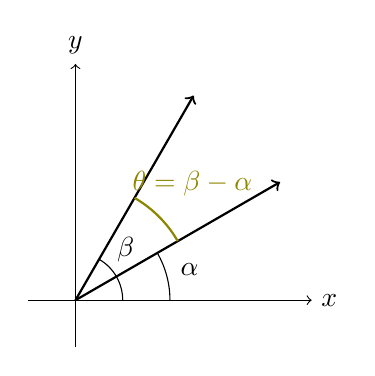
\begin{tikzpicture}[scale=3]
			% Draw axes
			\draw[->] (-0.2, 0) -- (1, 0) node[right] {$x$};
			\draw[->] (0, -0.2) -- (0, 1) node[above] {$y$};

			% Draw angle beta
			\draw[->, thick, black] (0,0) -- (30:1cm);
			\draw[->, thick, black] (0,0) -- (60:1cm);

			% % Mark angles (cosine)
			% Mark arc for be (smaller radius)
			\draw (0.4cm, 0) arc (0:30:0.4cm);  % arc for be (lower)
			\node at (15:0.5cm) {$\alpha$};

			% Mark arc for beta (larger radius)
			\draw (0.2cm, 0) arc (0:60:0.2cm);  % arc for beta
			\node at (45:0.3cm) {$\beta$};

			% Mark arc for theta (same radius as beta)
			\draw[thick, olive] (30:0.5cm) arc (30:60:0.5cm);  % arc for theta from be to beta
			\node[olive] at (45:0.7cm) {$\theta = \beta - \alpha $};

		\end{tikzpicture}
		\caption{Visualization of $\cos(\beta - \alpha) = \cos(\theta)$ in the unit circle.}
	\end{figure}

	\noindent\textnormal{For unit vectors, $\cos \theta = v \cdot w$.
		When $v$ and $w$ are not unit vectors, divide by their length to get $u = v/\|v\|$ and $U = u/\|u\|$ and turn them into unit vectors.}
\end{example}


\label{sec:vectors_and_linear_combination_end}